        \documentclass{standalone}
        \usepackage{tikz}
        \usetikzlibrary{arrows}
        \usepackage{amsmath}
        \usepackage{amsfonts}
        \begin{document}
        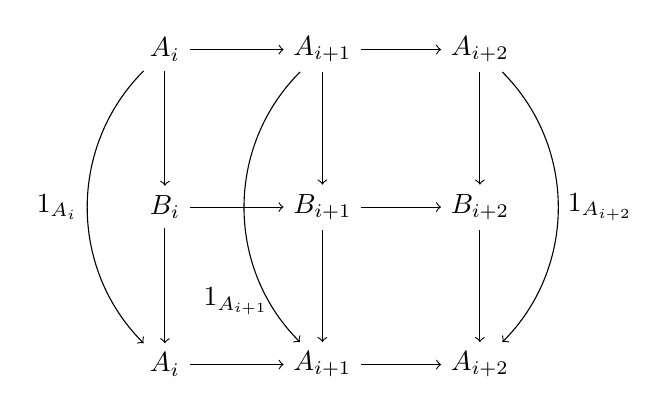
\begin{tikzpicture}

    \node (A1) at (-2,0) {$A_i$};
    \node (A2) at (0,0) {$A_{i+1}$};
    \node (A3) at (2,0) {$A_{i+2}$};
    \node (B1) at (-2,-2) {$B_i$};
    \node (B2) at (0,-2) {$B_{i+1}$};
    \node (B3) at (2,-2) {$B_{i+2}$};
    \node (A12) at (-2,-4) {$A_i$};
    \node (A22) at (0,-4) {$A_{i+1}$};
    \node (A32) at (2,-4) {$A_{i+2}$};
    \node at (-1.1,-3.2) {$1_{A_{i+1}}$};
    \draw[->] (A1) -- (A2);
    \draw[->] (A2) -- (A3);
    \draw[->] (B1) -- (B2);
    \draw[->] (B2) -- (B3);
    \draw[->] (A12) -- (A22);
    \draw[->] (A22) -- (A32);
    \draw[->] (A1) -- (B1);
    \draw[->] (A2) -- (B2);
    \draw[->] (A3) -- (B3);
    \draw[->] (B1) -- (A12);
    \draw[->] (B2) -- (A22);
    \draw[->] (B3) -- (A32);
    \draw[->] (A1) to [out=225,in=135] node[left] {$1_{A_i}$} (A12);
    \draw[->] (A2) to [out=225,in=135] (A22);
    \draw[->] (A3) to [out=315,in=45] node[right] {$1_{A_{i+2}}$} (A32);
        \end{tikzpicture}
        \end{document}
